% vim: set spell spelllang=en tw=100 et sw=4 sts=4 :

\documentclass{llncs}

% \usepackage{showframe}

\usepackage{microtype}                 % typographic perfection
\usepackage{complexity}                % \P, \NP etc
\usepackage{tikz}                      % For pretty pictures
\usepackage{amsmath}                   % \operatorname
\usepackage{amsfonts}                  % \mathbb
\usepackage{hyperref}                  % clicky links
\usepackage{cleveref}                  % no need to type Figure etc
\usepackage{gnuplot-lua-tikz}          % graphs
\usepackage[ruled,vlined]{algorithm2e} % algorithms (after cleverref!)
\usepackage{cite}                      % automatically sort mass cites
\usepackage[bottom]{footmisc}          % fix footnote + bottom figure on same page

\usetikzlibrary{arrows, shadows, calc, positioning, decorations, decorations.pathreplacing,
    patterns, matrix}

% lncs style
\crefname{algocf}{Algorithm}{Algorithms}
\Crefname{algocf}{Algorithm}{Algorithms}
\crefname{figure}{Fig.}{Figs.}
\Crefname{figure}{Fig.}{Figs.}
\crefname{table}{Table}{Tables}
\Crefname{table}{Table}{Tables}
\crefname{proposition}{Proposition}{Propositions}
\Crefname{proposition}{Proposition}{Propositions}

% pretty colours
\definecolor{uofgsandstone}{rgb}{0.321569, 0.278431, 0.231373}
\definecolor{uofgsunshine}{rgb}{1.0, 0.862745, 0.211765}
\definecolor{uofgcobalt}{rgb}{0, 0.615686, 0.92549}
\definecolor{uofglawn}{rgb}{0.517647, 0.741176, 0}
\definecolor{uofgthistle}{rgb}{0.584314, 0.070588, 0.447059}

\newcommand{\lineref}[1]{line~\ref{#1}}
\newcommand{\twolinesref}[2]{lines~\ref{#1} and~\ref{#2}}

\newcommand*\samethanks[1][\value{footnote}]{\footnotemark[#1]}

\title{Clique and Constraint Models for Maximum Common (Connected) Subgraph Problems}

\author{Ciaran McCreesh\thanks{This work was supported by the Engineering and Physical Sciences
    Research Council [grant number EP/K503058/1]}\inst{1} \and Samba Ndojh Ndiaye\thanks{This work
was supported by the ANR project SoLStiCe (ANR-13-BS02-0002-01)}\inst{2} \and Patrick
Prosser\inst{1} \and Christine Solnon\samethanks[2] \inst{3}}
\institute{University of Glasgow, Glasgow, Scotland \and
Universit\'e Lyon 1, LIRIS, UMR5205, F-69621, France  \and INSA-Lyon, LIRIS, UMR5205, F-69621, France}

\begin{document}

\maketitle

\begin{abstract}
    The maximum common subgraph problem is to find the largest subgraph common to two given graphs.
    This problem can be solved either by constraint-based search, or by reduction to the maximum
    clique problem. We evaluate these two approaches using modern algorithms. We also investigate a
    restricted branching approach for the connected version of the problem, show how to implement
    this in constraint-based and clique-inspired algorithms, and compare it to conventional
    propagation.
\end{abstract}

\section{Introduction}

\begin{figure}[b] % first page if possible
    \centering
    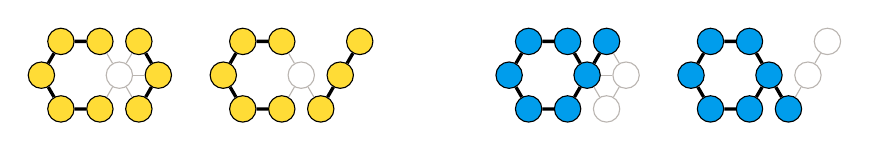
\begin{tikzpicture}[scale=0.33]%{{{
        \begin{scope}[rotate=90]
            \node[draw, circle, fill=uofgsunshine, inner sep=0.5pt, font=\normalsize] (M1) at (90:1.5) {\phantom{0}};
            \node[draw, circle, fill=uofgsunshine, inner sep=0.5pt, font=\normalsize] (M2) at (150:1.5) {\phantom{0}};
            \node[draw, circle, fill=uofgsunshine, inner sep=0.5pt, font=\normalsize] (M3) at (30:1.5) {\phantom{0}};
            \node[draw, circle, fill=uofgsunshine, inner sep=0.5pt, font=\normalsize] (M4) at (210:1.5) {\phantom{0}};
            \node[draw, circle, fill=uofgsunshine, inner sep=0.5pt, font=\normalsize] (M5) at (330:1.5) {\phantom{0}};
            \node[draw, circle, draw=uofgsandstone!40, fill=white, inner sep=0.5pt, font=\normalsize] (M6) at (270:1.5) {\phantom{0}};
            \node[draw, circle, fill=uofgsunshine, inner sep=0.5pt, font=\normalsize] (M7) at ($(210:1.5) + (M6)$) {\phantom{0}};
            \node[draw, circle, fill=uofgsunshine, inner sep=0.5pt, font=\normalsize] (M8) at ($(330:1.5) + (M6)$) {\phantom{0}};
            \node[draw, circle, fill=uofgsunshine, inner sep=0.5pt, font=\normalsize] (M9) at ($(270:1.5) + (M6)$) {\phantom{0}};

            \draw [very thick] (M1) -- (M2);
            \draw [very thick] (M2) -- (M4);
            \draw [very thick] (M3) -- (M5);
            \draw [color=uofgsandstone!40] (M4) -- (M6);
            \draw [color=uofgsandstone!40] (M5) -- (M6);
            \draw [very thick] (M3) -- (M1);
            \draw [color=uofgsandstone!40] (M6) -- (M7);
            \draw [color=uofgsandstone!40] (M6) -- (M8);
            \draw [color=uofgsandstone!40] (M6) -- (M9);
            \draw [very thick] (M7) -- (M9);
            \draw [very thick] (M8) -- (M9);
        \end{scope}

        \begin{scope}[xshift=7cm, rotate=90]
            \node[draw, circle, fill=uofgsunshine, inner sep=0.5pt, font=\normalsize] (M1) at (90:1.5) {\phantom{0}};
            \node[draw, circle, fill=uofgsunshine, inner sep=0.5pt, font=\normalsize] (M2) at (150:1.5) {\phantom{0}};
            \node[draw, circle, fill=uofgsunshine, inner sep=0.5pt, font=\normalsize] (M3) at (30:1.5) {\phantom{0}};
            \node[draw, circle, fill=uofgsunshine, inner sep=0.5pt, font=\normalsize] (M4) at (210:1.5) {\phantom{0}};
            \node[draw, circle, fill=uofgsunshine, inner sep=0.5pt, font=\normalsize] (M5) at (330:1.5) {\phantom{0}};
            \node[draw, circle, draw=uofgsandstone!40, fill=white, inner sep=0.5pt, font=\normalsize] (M6) at (270:1.5) {\phantom{0}};
            \node[draw, circle, fill=uofgsunshine, inner sep=0.5pt, font=\normalsize] (M7) at ($(210:1.5) + (M6)$) {\phantom{0}};
            \node[draw, circle, fill=uofgsunshine, inner sep=0.5pt, font=\normalsize] (M8) at ($(270:1.5) + (M6)$) {\phantom{0}};
            \node[draw, circle, fill=uofgsunshine, inner sep=0.5pt, font=\normalsize] (M9) at ($(330:1.5) + (M8)$) {\phantom{0}};

            \draw [very thick] (M1) -- (M2);
            \draw [very thick] (M2) -- (M4);
            \draw [very thick] (M3) -- (M5);
            \draw [color=uofgsandstone!40] (M4) -- (M6);
            \draw [color=uofgsandstone!40] (M5) -- (M6);
            \draw [very thick] (M3) -- (M1);
            \draw [color=uofgsandstone!40] (M6) -- (M7);
            \draw [very thick] (M7) -- (M8);
            \draw [very thick] (M8) -- (M9);
        \end{scope}

        \begin{scope}[xshift=18cm, rotate=90]
            \node[draw, circle, fill=uofgcobalt, inner sep=0.5pt, font=\normalsize] (M1) at (90:1.5) {\phantom{0}};
            \node[draw, circle, fill=uofgcobalt, inner sep=0.5pt, font=\normalsize] (M2) at (150:1.5) {\phantom{0}};
            \node[draw, circle, fill=uofgcobalt, inner sep=0.5pt, font=\normalsize] (M3) at (30:1.5) {\phantom{0}};
            \node[draw, circle, fill=uofgcobalt, inner sep=0.5pt, font=\normalsize] (M4) at (210:1.5) {\phantom{0}};
            \node[draw, circle, fill=uofgcobalt, inner sep=0.5pt, font=\normalsize] (M5) at (330:1.5) {\phantom{0}};
            \node[draw, circle, fill=uofgcobalt, inner sep=0.5pt, font=\normalsize] (M6) at (270:1.5) {\phantom{0}};
            \node[draw, circle, draw=uofgsandstone!40, fill=white, inner sep=0.5pt, font=\normalsize] (M7) at ($(210:1.5) + (M6)$) {\phantom{0}};
            \node[draw, circle, fill=uofgcobalt, inner sep=0.5pt, font=\normalsize] (M8) at ($(330:1.5) + (M6)$) {\phantom{0}};
            \node[draw, circle, draw=uofgsandstone!40, fill=white, inner sep=0.5pt, font=\normalsize] (M9) at ($(270:1.5) + (M6)$) {\phantom{0}};

            \draw [very thick] (M1) -- (M2);
            \draw [very thick] (M2) -- (M4);
            \draw [very thick] (M3) -- (M5);
            \draw [very thick] (M4) -- (M6);
            \draw [very thick] (M5) -- (M6);
            \draw [very thick] (M3) -- (M1);
            \draw [color=uofgsandstone!40] (M6) -- (M7);
            \draw [very thick] (M6) -- (M8);
            \draw [color=uofgsandstone!40] (M6) -- (M9);
            \draw [color=uofgsandstone!40] (M7) -- (M9);
            \draw [color=uofgsandstone!40] (M8) -- (M9);
        \end{scope}

        \begin{scope}[xshift=25cm, rotate=90]
            \node[draw, circle, fill=uofgcobalt, inner sep=0.5pt, font=\normalsize] (M1) at (90:1.5) {\phantom{0}};
            \node[draw, circle, fill=uofgcobalt, inner sep=0.5pt, font=\normalsize] (M2) at (150:1.5) {\phantom{0}};
            \node[draw, circle, fill=uofgcobalt, inner sep=0.5pt, font=\normalsize] (M3) at (30:1.5) {\phantom{0}};
            \node[draw, circle, fill=uofgcobalt, inner sep=0.5pt, font=\normalsize] (M4) at (210:1.5) {\phantom{0}};
            \node[draw, circle, fill=uofgcobalt, inner sep=0.5pt, font=\normalsize] (M5) at (330:1.5) {\phantom{0}};
            \node[draw, circle, fill=uofgcobalt, inner sep=0.5pt, font=\normalsize] (M6) at (270:1.5) {\phantom{0}};
            \node[draw, circle, fill=uofgcobalt, inner sep=0.5pt, font=\normalsize] (M7) at ($(210:1.5) + (M6)$) {\phantom{0}};
            \node[draw, circle, draw=uofgsandstone!40, fill=white, inner sep=0.5pt, font=\normalsize] (M8) at ($(270:1.5) + (M6)$) {\phantom{0}};
            \node[draw, circle, draw=uofgsandstone!40, fill=white, inner sep=0.5pt, font=\normalsize] (M9) at ($(330:1.5) + (M8)$) {\phantom{0}};

            \draw [very thick] (M1) -- (M2);
            \draw [very thick] (M2) -- (M4);
            \draw [very thick] (M3) -- (M5);
            \draw [very thick] (M4) -- (M6);
            \draw [very thick] (M5) -- (M6);
            \draw [very thick] (M3) -- (M1);
            \draw [very thick] (M6) -- (M7);
            \draw [draw=uofgsandstone!40] (M7) -- (M8);
            \draw [draw=uofgsandstone!40] (M8) -- (M9);
        \end{scope}
\end{tikzpicture}
\caption{A maximum common induced subgraph of the first two graphs has eight vertices, shaded.
However, if we require the common subgraph to be connected, only seven vertices may be
selected---one way to do this is shown in the third and fourth graphs.}\label{figure:mcsexample}
\end{figure}

Maximum common subgraph problems arise in biology and chemistry
\cite{DBLP:journals/jcamd/RaymondW02a,Ehrlich:2011}, computer vision ?? what should we cite?, ??
anything else?, both directly and as a way of measuring the similarity or difference between two
graphs \cite{DBLP:journals/prl/Bunke97,DBLP:journals/prl/FernandezV01,KriegeThesis}. We illustrate
this in \cref{figure:mcsexample}, and define the problem formally below.

\subsection{Definitions and Notation}

We will be working with graphs which may be directed, which may have labels associated with
vertices, edges, or both, and which may contain loops. To simplify notation, we will work with a
single definition throughout: we define a \emph{graph} $G = (V, \ell, e)$ to be a set of vertices
$V$, a vertex labelling function $\ell : V \rightarrow \mathbb{N}$, and an edge labelling function
$e : V \times V \rightarrow \mathbb{N} \cup \{ \bot \}$. To represent graphs without vertex (or
edge) labels, we just pick our favourite number and give it to every vertex (or edge). We also use a
distinct label $\bot$ to represent the \emph{lack of} an edge between two vertices.  We write
$\operatorname{V}(G)$ for $V$, and $\operatorname{N}(G, v)$ for the \emph{undirected neighbourhood}
of a vertex $v$ (that is, the set of vertices $w$ such that either $e(v, w) \ne \bot$ or $e(w, v)
\ne \bot$); a vertex is \emph{isolated} if its neighbourhood is empty. A \emph{path} between two
vertices $v$ and $w$ is a sequence of $n$ vertices $v = v_1, v_2, \ldots, v_n = w$ such that for
each $m \in \{ 1 \ldots n - 1 \}$, $e(v_m, v_{m + 1}) \ne \bot$.  A graph is \emph{connected} if a
path exists between each distinct pair of vertices.

Given two graphs $G_1 = (V_1, \ell_1, e_1)$ and $G_2 = (V_2, \ell_2, e_2)$, we say two pairs of
vertices $(v_1, w_1) \in \operatorname{V}(G_1) \times \operatorname{V}(G_1)$ and $(v_2, w_2) \in
\operatorname{V}(G_2) \times \operatorname{V}(G_2)$ are \emph{compatible}, written $(v_1, w_1)
\simeq (v_2, w_2)$, if both $e_1(v_1, w_1) = e_2(v_2, w_2)$ and $e_1(w_1, v_1) = e_2(w_2, v_2)$. We
say two vertices $v \in \operatorname{V}(G_1)$ and $w \in \operatorname{V}(G_2)$ are
\emph{compatible}, written $v \simeq w$, if $\ell_1(v) = \ell_2(w)$ and $(v, v) \simeq (w, w)$.

An \emph{induced subgraph isomorphism} from a graph $G$ to a graph $H$ is an injective function $i :
\operatorname{V}(G) \rightarrow \operatorname{V}(H)$ such that for every vertex $v \in
\operatorname{V}(G)$, $v \simeq i(v)$, and for every pair of vertices $(v, w) \in
\operatorname{V}(G) \times \operatorname{V}(G)$, $(v, w) \simeq (i(v), i(w))$. A \emph{common
induced subgraph isomorphism} between two graphs $G_1$ and $G_2$ is a graph $G$, together with a
pair of induced subgraph isomorphisms $i_1 : G \rightarrow G_1$ and $i_2 : G \rightarrow G_2$. A
\emph{common induced subgraph} of $G_1$ and $G_2$ is a graph $G$ which has a common subgraph
isomorphism to $G_1$ and $G_2$. A \emph{maximum common (connected) induced subgraph} is a common
(connected) induced subgraph with the largest possible number of vertices.  (The distinction between
a common subgraph and a common subgraph isomorphism is relevant when counting distinct solutions,
which we do not consider in this paper; in \cref{figure:mcsexample} on the left, there is only one
maximum common subgraph, but four different maximum common subgraph isomorphisms are possible.)

There is also a non-induced version of these problems, which is commonly known as the \emph{maximum
common partial subgraph} problem: here, if $e(v, w) = \bot$, then $e_1(i_1(v), i_1(w))$ and
$e_2(i_2(v), i_2(w))$ may take any value, and we must maximise the number of non-$\bot$ vertex pairs
(i.e.\ edges) in $G$ instead (it is not entirely clear what the objective should be in directed
graphs, or when loops are present). We restrict ourselves to the induced version in this paper (??
we could do a journal version, because the clique side is rather involved\ldots).

\subsection{Existing Approaches}

One approach to maximum common subgraph problems is via constraint programming
\cite{DBLP:conf/mco/VismaraV08,DBLP:conf/cp/NdiayeS11}. The models are based upon constructing an
injective mapping from the vertices of one graph (typically the smaller) to the other, in a similar
manner to subgraph isomorphism algorithms
\cite{DBLP:journals/ai/Solnon10,DBLP:conf/cp/AudemardLMGP14,DBLP:conf/cp/McCreeshP15}. However, to
allow for a partial mapping, a special $\bot$ value is added to each domain (and so we are
constructing a maximum common subgraph isomorphism, where the common subgraph is implicitly the
subgraph of the first graph given by taking the vertices which are not assigned to $\bot$, and the
first subgraph isomorphism is the inclusion map). The objective is then to minimise the number of
variables given the $\bot$ value---for best results, a special propagator for the injectivity
condition is used, which simultaneously enforces that all variables taking non-$\bot$ are different,
and restricts the number of $\bot$ values which may be used based upon the objective
\cite{DBLP:conf/cp/PetitRB01}.  Unfortunately, the addition of $\bot$ also invalidates many of the
invariants used for subgraph isomorphism---we may no longer reason using the degree of vertices, for
example, and so maximum common subgraph problems can be much more challenging in practice.

Another widely studied approach is to reduce the problem to finding a maximum clique (or sometimes,
equivalently, an independent set or a vertex cover) in an association graph (which we describe
below). Conventional wisdom is that this approach is less effective in practice, but previous
experimental evaluations have used weak clique algorithms, or even maximal clique enumeration
algorithms. Maximum clique algorithms are an active research area
\cite{DBLP:conf/dmtcs/TomitaS03,DBLP:journals/jgo/TomitaK07,DBLP:conf/walcom/TomitaSHTW10,DBLP:journals/cor/SegundoRJ11,DBLP:journals/algorithms/Prosser12,DBLP:journals/ol/SegundoMRH13,DBLP:conf/ictai/LiFX13,DBLP:journals/cor/SegundoT14,DBLP:conf/lion/SegundoLB14,DBLP:conf/cp/McCreeshP14,DBLP:journals/jco/BatsynGMP14,DBLP:journals/cor/SegundoNB15,DBLP:conf/lion/NikolaevBS15,DBLP:conf/lion/LiJX15,DBLP:journals/jcc/KoncDTRJ12,DBLP:journals/algorithms/McCreeshP13,DBLP:journals/topc/McCreeshP15,DBLP:journals/cor/SegundoLP16},
and so the first half of this paper re-evaluates the association graph approach using a modern
algorithm.

(Other approaches have been tried, including mixed integer programming
\cite{DBLP:journals/anor/PivaS12}; SAT encodings seem to struggle even for subgraph isomorphism??
cite IJCAI if it's not rejected?.)

An interesting variant of the maximum common subgraph problem requires the selected subgraph to be
connected
\cite{DBLP:journals/tcs/Koch01,DBLP:journals/jcamd/RaymondW02a,DBLP:conf/mco/VismaraV08,Ehrlich:2011}.
Adding the connectedness requirement makes certain special cases solvable in polynomial time,
including outerplanar graphs of bounded degree \cite{DBLP:journals/algorithms/AkutsuT13} and trees
\cite{DBLP:journals/corr/DroschinskyKM16}, but the general case remains \NP-hard. The second half of
this paper looks at this variant on arbitrary graphs. In principle, for a constraint programming
approach, we may simply add a ``forms a connected graph'' global constraint to the model
\cite{Brown:2005,DBLP:conf/cp/DoomsDD05,DBLP:conf/cp/QuesadaRD05}. Alternatively, we could use a
special branching rule to maintain connectedness during search ?? cite. We see that using both
approaches together gives best results ?? does it?.  We also explain how to adapt this branching
rule to run inside a modern clique-like algorithm, to solve the problem via an association graph.

?? Summary, association graph is better when edges have labels.

\subsection{Datasets}

\cite{DBLP:journals/prl/SantoFSV03,DBLP:journals/jgaa/ConteFV07}

?? More? Can we scale to some of the SIP graphs?

\section{Re-Evaluating the Clique Model}

Previous experimental work has used a maximal clique enumeration algorithm, even for the
maximisation problem. ?? check this! I recall someone using a bad max clique algorithm too.
\cite{DBLP:conf/sspr/BunkeFGSV02,DBLP:journals/jgaa/ConteFV07}

We instead use a maximum clique algorithm.

Also sparse stuff, but association graphs aren't sparse enough.

Say which clique algorithm we're using.

\subsection{Reduction to Maximum Clique in an Association Graph}

Explain association graph \cref{figure:association}, cite history, connections to microstructure
\cite{DBLP:conf/aaai/Jegou93a}.

Discuss how edge labels, vertex labels, directed edges, etc, are handled. Note that we can generally
only handle very local side constraints, or injectivity (which is decomposable).

\begin{figure}[tb]
    \centering
    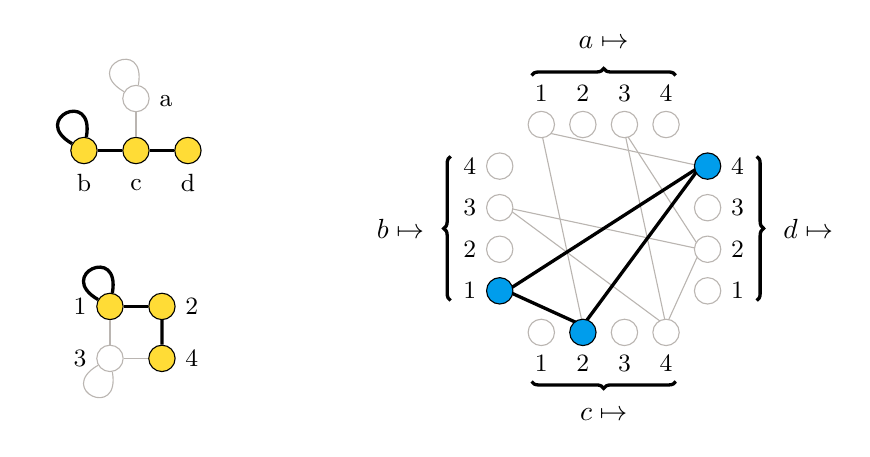
\begin{tikzpicture}[scale=0.33]%{{{
        \begin{scope}
            \node[draw, circle, fill=white, draw=uofgsandstone!40, inner sep=0.5pt, font=\normalsize] (Ma) at (2, 10) {\phantom{0}};
            \node[draw, circle, fill=uofgsunshine, inner sep=0.5pt, font=\normalsize] (Mb) at (0, 8) {\phantom{0}};
            \node[draw, circle, fill=uofgsunshine, inner sep=0.5pt, font=\normalsize] (Mc) at (2, 8) {\phantom{0}};
            \node[draw, circle, fill=uofgsunshine, inner sep=0.5pt, font=\normalsize] (Md) at (4, 8) {\phantom{0}};

            \node [right = 0 of Ma, font=\small] { \vphantom{0}a };
            \node [below = 0 of Mb, font=\small] { \vphantom{0}b };
            \node [below = 0 of Mc, font=\small] { \vphantom{0}c };
            \node [below = 0 of Md, font=\small] { \vphantom{0}d };

            \draw [very thick] (Mb) -- (Mc);
            \draw [very thick] (Mc) -- (Md);
            \draw [color=uofgsandstone!40] (Ma) -- (Mc);
            \draw [color=uofgsandstone!40] (Ma) to [out=150, in=80, looseness=8] (Ma);
            \draw [very thick] (Mb) to [out=150, in=80, looseness=8] (Mb);
        \end{scope}

        \begin{scope}
            \node[draw, circle, fill=uofgsunshine, inner sep=0.5pt, font=\normalsize] (M1) at (1, 2) {\phantom{0}};
            \node[draw, circle, fill=uofgsunshine, inner sep=0.5pt, font=\normalsize] (M2) at (3, 2) {\phantom{0}};
            \node[draw, circle, fill=white, draw=uofgsandstone!40, inner sep=0.5pt, font=\normalsize] (M3) at (1, 0) {\phantom{0}};
            \node[draw, circle, fill=uofgsunshine, inner sep=0.5pt, font=\normalsize] (M4) at (3, 0) {\phantom{0}};

            \node [left = 0 of M1, font=\small] { \vphantom{0}1 };
            \node [right = 0 of M2, font=\small] { \vphantom{0}2 };
            \node [left = 0 of M3, font=\small] { \vphantom{0}3 };
            \node [right = 0 of M4, font=\small] { \vphantom{0}4 };

            \draw [very thick] (M1) -- (M2);
            \draw [very thick] (M2) -- (M4);
            \draw [color=uofgsandstone!40] (M3) -- (M4);
            \draw [color=uofgsandstone!40] (M1) -- (M3);

            \draw [color=uofgsandstone!40] (M3) to [out=280, in=210, looseness=8] (M3);
            \draw [very thick] (M1) to [out=150, in=80, looseness=8] (M1);
        \end{scope}

        \begin{scope}[xshift=15cm]
            \node[draw, circle, fill=white, draw=uofgsandstone!40, inner sep=0.5pt, font=\normalsize] (Ma1) at (2.6, 9) {\phantom{0}};
            \node[draw, circle, fill=white, draw=uofgsandstone!40, inner sep=0.5pt, font=\normalsize] (Ma2) at (4.2, 9) {\phantom{0}};
            \node[draw, circle, fill=white, draw=uofgsandstone!40, inner sep=0.5pt, font=\normalsize] (Ma3) at (5.8, 9) {\phantom{0}};
            \node[draw, circle, fill=white, draw=uofgsandstone!40, inner sep=0.5pt, font=\normalsize] (Ma4) at (7.4, 9) {\phantom{0}};
            \node [above = 0 of Ma1, font=\small] { \vphantom{0}1 };
            \node [above = 0 of Ma2, font=\small] { \vphantom{0}2 };
            \node [above = 0 of Ma3, font=\small] { \vphantom{0}3 };
            \node [above = 0 of Ma4, font=\small] { \vphantom{0}4 };

            \draw [decorate, decoration={brace, raise=0.5cm}, very thick] (Ma1.north west) -- (Ma4.north east)
            node [midway, above=0.7cm] { $a \mapsto$ };

            \node[draw, circle, fill=uofgcobalt, inner sep=0.5pt, font=\normalsize] (Mb1) at (1, 2.6) {\phantom{0}};
            \node[draw, circle, fill=white, draw=uofgsandstone!40, inner sep=0.5pt, font=\normalsize] (Mb2) at (1, 4.2) {\phantom{0}};
            \node[draw, circle, fill=white, draw=uofgsandstone!40, inner sep=0.5pt, font=\normalsize] (Mb3) at (1, 5.8) {\phantom{0}};
            \node[draw, circle, fill=white, draw=uofgsandstone!40, inner sep=0.5pt, font=\normalsize] (Mb4) at (1, 7.4) {\phantom{0}};
            \node [left = 0 of Mb1, font=\small] { \vphantom{0}1 };
            \node [left = 0 of Mb2, font=\small] { \vphantom{0}2 };
            \node [left = 0 of Mb3, font=\small] { \vphantom{0}3 };
            \node [left = 0 of Mb4, font=\small] { \vphantom{0}4 };

            \draw [decorate, decoration={brace, raise=0.5cm}, very thick] (Mb1.south west) -- (Mb4.north west)
            node [midway, left=0.7cm] { $b \mapsto$ };

            \node[draw, circle, fill=white, draw=uofgsandstone!40, inner sep=0.5pt, font=\normalsize] (Mc1) at (2.6, 1) {\phantom{0}};
            \node[draw, circle, fill=uofgcobalt, inner sep=0.5pt, font=\normalsize] (Mc2) at (4.2, 1) {\phantom{0}};
            \node[draw, circle, fill=white, draw=uofgsandstone!40, inner sep=0.5pt, font=\normalsize] (Mc3) at (5.8, 1) {\phantom{0}};
            \node[draw, circle, fill=white, draw=uofgsandstone!40, inner sep=0.5pt, font=\normalsize] (Mc4) at (7.4, 1) {\phantom{0}};
            \node [below = 0 of Mc1, font=\small] { \vphantom{0}1 };
            \node [below = 0 of Mc2, font=\small] { \vphantom{0}2 };
            \node [below = 0 of Mc3, font=\small] { \vphantom{0}3 };
            \node [below = 0 of Mc4, font=\small] { \vphantom{0}4 };

            \draw [decorate, decoration={brace, raise=0.5cm}, very thick] (Mc4.south east) -- (Mc1.south west)
            node [midway, below=0.7cm] { $c \mapsto$ };

            \node[draw, circle, fill=white, draw=uofgsandstone!40, inner sep=0.5pt, font=\normalsize] (Md1) at (9, 2.6) {\phantom{0}};
            \node[draw, circle, fill=white, draw=uofgsandstone!40, inner sep=0.5pt, font=\normalsize] (Md2) at (9, 4.2) {\phantom{0}};
            \node[draw, circle, fill=white, draw=uofgsandstone!40, inner sep=0.5pt, font=\normalsize] (Md3) at (9, 5.8) {\phantom{0}};
            \node[draw, circle, fill=uofgcobalt, inner sep=0.5pt, font=\normalsize] (Md4) at (9, 7.4) {\phantom{0}};
            \node [right = 0 of Md1, font=\small] { \vphantom{0}1 };
            \node [right = 0 of Md2, font=\small] { \vphantom{0}2 };
            \node [right = 0 of Md3, font=\small] { \vphantom{0}3 };
            \node [right = 0 of Md4, font=\small] { \vphantom{0}4 };

            \draw [decorate, decoration={brace, raise=0.5cm}, very thick] (Md4.north east) -- (Md1.south east)
            node [midway, right=0.7cm] { $d \mapsto$ };

            \begin{scope}[on background layer]
                \draw [draw=uofgsandstone!40] ($(Ma1.south)!0.5!(Ma1)$) -- ($(Md4.west)!0.5!(Md4)$);
                \draw [draw=uofgsandstone!40] ($(Ma1.south)!0.5!(Ma1)$) -- ($(Mc2.north)!0.5!(Mc2)$);
                \draw [draw=uofgsandstone!40] ($(Ma3.south)!0.5!(Ma3)$) -- ($(Mc4.north)!0.5!(Mc4)$);
                \draw [draw=uofgsandstone!40] ($(Mb3.east)!0.5!(Mb3)$) -- ($(Mc4.north)!0.5!(Mc4)$);
                \draw [draw=uofgsandstone!40] ($(Md2.west)!0.5!(Md2)$) -- ($(Mc4.north)!0.5!(Mc4)$);
                \draw [draw=uofgsandstone!40] ($(Md2.west)!0.5!(Md2)$) -- ($(Ma3.south)!0.5!(Ma3)$);
                \draw [draw=uofgsandstone!40] ($(Md2.west)!0.5!(Md2)$) -- ($(Mb3.east)!0.5!(Mb3)$);
                \draw [very thick] ($(Mb1.east)!0.5!(Mb1)$) -- ($(Mc2.north)!0.5!(Mc2)$);
                \draw [very thick] ($(Mb1.east)!0.5!(Mb1)$) -- ($(Md4.west)!0.5!(Md4)$);
                \draw [very thick] ($(Mc2.north)!0.5!(Mc2)$) -- ($(Md4.west)!0.5!(Md4)$);
        \end{scope}
        \end{scope}

    \end{tikzpicture}

    \caption{A maximum common induced subgraph between the two graphs on the left has three
        vertices---one solution is highlighted. On the right, the association graph encoding: the
        highlighted clique of size three shows the same solution. In practice the isolated vertices
        (corresponding to assignments between incompatible vertices, which are unary constraints) would be
        omitted.}\label{figure:association}
\end{figure}

?? Discuss the partial version briefly, cite the reduction.

\subsection{Experimental Evaluation}

\cref{figure:unconnected-33}

\cref{figure:unconnected-plain}

?? Break this down more by family, size, etc.

\begin{figure}[p]
    \centering
    \input{gen-graph-unconnected-33}
    \caption{Clique versus constraint programming, 33\% labelled. On the top, the cumulative
    number of instances solved by each approach, in under a certain time. On the bottom, an
    instance-by-instance comparison of the two approaches: the colour at a point indicates the
    number of instances with these runtimes.} \label{figure:unconnected-33}
\end{figure}

\begin{figure}[p]
    \centering
    \input{gen-graph-unconnected-33-breakdown}
    \caption{Clique versus constraint programming, 33\% labelled, broken down by family.}
        \label{figure:unconnected-33-breakdown}
\end{figure}

\begin{figure}[p]
    \centering
    \input{gen-graph-unconnected-plain}
    \caption{Clique versus constraint programming, undirected, unlabelled. On the top, the cumulative
    number of instances solved by each approach, in under a certain time. On the bottom, an
        instance-by-instance comparison of the two approaches: the colour at a point indicates the
    number of instances with these runtimes.} \label{figure:unconnected-plain}
\end{figure}

\begin{figure}[p]
    \centering
    \input{gen-graph-unconnected-plain-breakdown}
    \caption{Clique versus constraint programming, undirected, unlabelled, broken down by family.}
        \label{figure:unconnected-plain-breakdown}
\end{figure}

\subsection{Filtering from Edge Labels}

\subsection{Parallel Search}

\cite{DBLP:journals/jcc/KoncDTRJ12,DBLP:journals/algorithms/McCreeshP13,DBLP:journals/topc/McCreeshP15,DBLP:journals/cor/SegundoLP16}

?? Stuff on EHPs, how work stealing matters here too \cite{DBLP:journals/jco/BatsynGMP14}

\section{Find Maximum Common Connected Subgraphs}

Connectedness is not hereditary, but can be built up one vertex at a time. Alternatively,
connectedness is a constraint.

\subsection{Connectedness as a Constraint}

Connectedness \cite{Brown:2005}

Reachability \cite{DBLP:conf/cp/DoomsDD05,DBLP:conf/cp/QuesadaRD05}

\subsection{Connectedness via Restricted Branching}

\begin{figure}[tb]
    \newcounter{stepcounter}
    \centering
    \begin{tikzpicture}[scale=0.33]%{{{
        \begin{scope}
            \node[draw, circle, fill=white, inner sep=0.5pt, font=\normalsize] (Ma) at (0, 4) {\phantom{0}};
            \node[draw, circle, fill=white, inner sep=0.5pt, font=\normalsize] (Mb) at (0, 2) {\phantom{0}};
            \node[draw, circle, fill=white, inner sep=0.5pt, font=\normalsize] (Mc) at (2, 2) {\phantom{0}};
            \node[draw, circle, fill=white, inner sep=0.5pt, font=\normalsize] (Md) at (0, 0) {\phantom{0}};
            \node[draw, circle, fill=white, inner sep=0.5pt, font=\normalsize] (Me) at (2, 0) {\phantom{0}};

            \node [left = 0 of Ma, font=\small] { \vphantom{0}a };
            \node [left = 0 of Mb, font=\small] { \vphantom{0}b };
            \node [right = 0 of Mc, font=\small] { \vphantom{0}c };
            \node [left = 0 of Md, font=\small] { \vphantom{0}d };
            \node [right = 0 of Me, font=\small] { \vphantom{0}e };

            \draw [draw=uofgsandstone!40] (Ma) -- (Mb);
            \draw [draw=uofgsandstone!40] (Ma) -- (Mc);
            \draw [draw=uofgsandstone!40] (Mb) -- (Mc);
            \draw [draw=uofgsandstone!40] (Mb) -- (Md);
            \draw [draw=uofgsandstone!40] (Mc) -- (Me);

            \node[draw, circle, fill=white, inner sep=0.5pt, font=\normalsize] (M1) at (5.6, 4) {\phantom{0}};
            \node[draw, circle, fill=white, inner sep=0.5pt, font=\normalsize] (M2) at (7.6, 4) {\phantom{0}};
            \node[draw, circle, fill=white, inner sep=0.5pt, font=\normalsize] (M3) at (5.6, 2) {\phantom{0}};
            \node[draw, circle, fill=white, inner sep=0.5pt, font=\normalsize] (M4) at (7.6, 2) {\phantom{0}};
            \node[draw, circle, fill=white, inner sep=0.5pt, font=\normalsize] (M5) at (5.6, 0) {\phantom{0}};

            \node [left = 0 of M1, font=\small] { \vphantom{0}1 };
            \node [right = 0 of M2, font=\small] { \vphantom{0}2 };
            \node [left = 0 of M3, font=\small] { \vphantom{0}3 };
            \node [right = 0 of M4, font=\small] { \vphantom{0}4 };
            \node [left = 0 of M5, font=\small] { \vphantom{0}5 };

            \draw [color=uofgsandstone!40] (M1) -- (M2);
            \draw [color=uofgsandstone!40] (M1) -- (M3);
            \draw [color=uofgsandstone!40] (M2) -- (M4);
            \draw [color=uofgsandstone!40] (M3) -- (M4);

            \node [anchor=base, yshift=-2.2cm] at ($(Ma)!0.5!(M2)$) {
                \stepcounter{stepcounter}\roman{stepcounter}) Initial problem };
        \end{scope}

        \begin{scope}[xshift=13cm]
            \node[draw, circle, fill=uofgsunshine, inner sep=0.5pt, font=\normalsize] (Ma) at (0, 4) {\phantom{0}};
            \node[draw, circle, fill=white, inner sep=0.5pt, font=\normalsize] (Mb) at (0, 2) {\phantom{0}};
            \node[draw, circle, fill=white, inner sep=0.5pt, font=\normalsize] (Mc) at (2, 2) {\phantom{0}};
            \node[draw, dotted, circle, fill=white, inner sep=0.5pt, font=\normalsize] (Md) at (0, 0) {\phantom{0}};
            \node[draw, dotted, circle, fill=white, inner sep=0.5pt, font=\normalsize] (Me) at (2, 0) {\phantom{0}};

            \node [left = 0 of Ma, font=\small] { \vphantom{0}a };
            \node [left = 0 of Mb, font=\small] { \vphantom{0}b };
            \node [right = 0 of Mc, font=\small] { \vphantom{0}c };
            \node [left = 0 of Md, font=\small] { \vphantom{0}d };
            \node [right = 0 of Me, font=\small] { \vphantom{0}e };

            \draw [draw=uofgsandstone!40] (Ma) -- (Mb);
            \draw [draw=uofgsandstone!40] (Ma) -- (Mc);
            \draw [draw=uofgsandstone!40] (Mb) -- (Mc);
            \draw [dotted] (Mb) -- (Md);
            \draw [dotted] (Mc) -- (Me);

            \node[draw, circle, fill=uofgsunshine, inner sep=0.5pt, font=\normalsize] (M1) at (5.6, 4) {\phantom{0}};
            \node[draw, circle, fill=white, inner sep=0.5pt, font=\normalsize] (M2) at (7.6, 4) {\phantom{0}};
            \node[draw, circle, fill=white, inner sep=0.5pt, font=\normalsize] (M3) at (5.6, 2) {\phantom{0}};
            \node[draw, circle, fill=white, inner sep=0.5pt, font=\normalsize] (M4) at (7.6, 2) {\phantom{0}};
            \node[draw, circle, fill=white, inner sep=0.5pt, font=\normalsize] (M5) at (5.6, 0) {\phantom{0}};

            \node [left = 0 of M1, font=\small] { \vphantom{0}1 };
            \node [right = 0 of M2, font=\small] { \vphantom{0}2 };
            \node [left = 0 of M3, font=\small] { \vphantom{0}3 };
            \node [right = 0 of M4, font=\small] { \vphantom{0}4 };
            \node [left = 0 of M5, font=\small] { \vphantom{0}5 };

            \draw [color=uofgsandstone!40] (M1) -- (M2);
            \draw [color=uofgsandstone!40] (M1) -- (M3);
            \draw [color=uofgsandstone!40] (M2) -- (M4);
            \draw [color=uofgsandstone!40] (M3) -- (M4);

            \node [anchor=base, yshift=-2.2cm] at ($(Ma)!0.5!(M2)$) {
                \stepcounter{stepcounter}\roman{stepcounter}) Trying $a \mapsto 1$ };
        \end{scope}

        \begin{scope}[xshift=26cm]
            \node[draw, circle, fill=uofgsunshine, inner sep=0.5pt, font=\normalsize] (Ma) at (0, 4) {\phantom{0}};
            \node[draw, circle, fill=uofgcobalt, inner sep=0.5pt, font=\normalsize] (Mb) at (0, 2) {\phantom{0}};
            \node[draw, circle, fill=white, draw=uofgsandstone!40, inner sep=0.5pt, font=\normalsize] (Mc) at (2, 2) {\phantom{0}};
            \node[draw, circle, fill=white, inner sep=0.5pt, font=\normalsize] (Md) at (0, 0) {\phantom{0}};
            \node[draw, dotted, circle, fill=white, inner sep=0.5pt, font=\normalsize] (Me) at (2, 0) {\phantom{0}};

            \node [left = 0 of Ma, font=\small] { \vphantom{0}a };
            \node [left = 0 of Mb, font=\small] { \vphantom{0}b };
            \node [right = 0 of Mc, font=\small] { \vphantom{0}c };
            \node [left = 0 of Md, font=\small] { \vphantom{0}d };
            \node [right = 0 of Me, font=\small] { \vphantom{0}e };

            \draw [very thick] (Ma) -- (Mb);
            \draw [color=uofgsandstone!40] (Ma) -- (Mc);
            \draw [color=uofgsandstone!40] (Mb) -- (Mc);
            \draw [color=uofgsandstone!40] (Mb) -- (Md);
            \draw [color=uofgsandstone!40] (Mc) -- (Me);

            \node[draw, circle, fill=uofgsunshine, inner sep=0.5pt, font=\normalsize] (M1) at (5.6, 4) {\phantom{0}};
            \node[draw, circle, fill=uofgcobalt, inner sep=0.5pt, font=\normalsize] (M2) at (7.6, 4) {\phantom{0}};
            \node[draw, circle, fill=white, inner sep=0.5pt, font=\normalsize] (M3) at (5.6, 2) {\phantom{0}};
            \node[draw, circle, fill=white, inner sep=0.5pt, font=\normalsize] (M4) at (7.6, 2) {\phantom{0}};
            \node[draw, circle, fill=white, inner sep=0.5pt, font=\normalsize] (M5) at (5.6, 0) {\phantom{0}};

            \node [left = 0 of M1, font=\small] { \vphantom{0}1 };
            \node [right = 0 of M2, font=\small] { \vphantom{0}2 };
            \node [left = 0 of M3, font=\small] { \vphantom{0}3 };
            \node [right = 0 of M4, font=\small] { \vphantom{0}4 };
            \node [left = 0 of M5, font=\small] { \vphantom{0}5 };

            \draw [very thick] (M1) -- (M2);
            \draw [color=uofgsandstone!40] (M1) -- (M3);
            \draw [color=uofgsandstone!40] (M2) -- (M4);
            \draw [color=uofgsandstone!40] (M3) -- (M4);

            \node [anchor=base, yshift=-2.2cm] at ($(Ma)!0.5!(M2)$) {
                \stepcounter{stepcounter}\roman{stepcounter}) Trying $b \mapsto 2$ };
        \end{scope}

        \begin{scope}[yshift=-9cm]
            \node[draw, circle, fill=uofgsunshine, inner sep=0.5pt, font=\normalsize] (Ma) at (0, 4) {\phantom{0}};
            \node[draw, circle, fill=uofgcobalt, inner sep=0.5pt, font=\normalsize] (Mb) at (0, 2) {\phantom{0}};
            \node[draw, circle, fill=white, draw=uofgsandstone!40, inner sep=0.5pt, font=\normalsize] (Mc) at (2, 2) {\phantom{0}};
            \node[draw, circle, fill=uofgthistle, inner sep=0.5pt, font=\normalsize] (Md) at (0, 0) {\phantom{0}};
            \node[draw, dotted, circle, fill=white, inner sep=0.5pt, font=\normalsize] (Me) at (2, 0) {\phantom{0}};

            \node [left = 0 of Ma, font=\small] { \vphantom{0}a };
            \node [left = 0 of Mb, font=\small] { \vphantom{0}b };
            \node [right = 0 of Mc, font=\small] { \vphantom{0}c };
            \node [left = 0 of Md, font=\small] { \vphantom{0}d };
            \node [right = 0 of Me, font=\small] { \vphantom{0}e };

            \draw [very thick] (Ma) -- (Mb);
            \draw [color=uofgsandstone!40] (Ma) -- (Mc);
            \draw [color=uofgsandstone!40] (Mb) -- (Mc);
            \draw [very thick] (Mb) -- (Md);
            \draw [color=uofgsandstone!40] (Mc) -- (Me);

            \node[draw, circle, fill=uofgsunshine, inner sep=0.5pt, font=\normalsize] (M1) at (5.6, 4) {\phantom{0}};
            \node[draw, circle, fill=uofgcobalt, inner sep=0.5pt, font=\normalsize] (M2) at (7.6, 4) {\phantom{0}};
            \node[draw, circle, fill=white, inner sep=0.5pt, font=\normalsize] (M3) at (5.6, 2) {\phantom{0}};
            \node[draw, circle, fill=uofgthistle, inner sep=0.5pt, font=\normalsize] (M4) at (7.6, 2) {\phantom{0}};
            \node[draw, circle, fill=white, inner sep=0.5pt, font=\normalsize] (M5) at (5.6, 0) {\phantom{0}};

            \node [left = 0 of M1, font=\small] { \vphantom{0}1 };
            \node [right = 0 of M2, font=\small] { \vphantom{0}2 };
            \node [left = 0 of M3, font=\small] { \vphantom{0}3 };
            \node [right = 0 of M4, font=\small] { \vphantom{0}4 };
            \node [left = 0 of M5, font=\small] { \vphantom{0}5 };

            \draw [very thick] (M1) -- (M2);
            \draw [color=uofgsandstone!40] (M1) -- (M3);
            \draw [very thick] (M2) -- (M4);
            \draw [color=uofgsandstone!40] (M3) -- (M4);

            \node [anchor=base, yshift=-2.2cm] at ($(Ma)!0.5!(M2)$) {
                \stepcounter{stepcounter}\roman{stepcounter}) Trying $d \mapsto 4$ };
        \end{scope}

        \begin{scope}[xshift=13cm, yshift=-9cm]
            \node[draw, circle, fill=uofgsunshine, inner sep=0.5pt, font=\normalsize] (Ma) at (0, 4) {\phantom{0}};
            \node[draw, circle, fill=uofgcobalt, inner sep=0.5pt, font=\normalsize] (Mb) at (0, 2) {\phantom{0}};
            \node[draw, circle, fill=white, draw=uofgsandstone!40, inner sep=0.5pt, font=\normalsize] (Mc) at (2, 2) {\phantom{0}};
            \node[draw, circle, fill=uofgthistle, inner sep=0.5pt, font=\normalsize] (Md) at (0, 0) {\phantom{0}};
            \node[draw, circle, fill=white, draw=uofgsandstone!40, inner sep=0.5pt, font=\normalsize] (Me) at (2, 0) {\phantom{0}};

            \node [left = 0 of Ma, font=\small] { \vphantom{0}a };
            \node [left = 0 of Mb, font=\small] { \vphantom{0}b };
            \node [right = 0 of Mc, font=\small] { \vphantom{0}c };
            \node [left = 0 of Md, font=\small] { \vphantom{0}d };
            \node [right = 0 of Me, font=\small] { \vphantom{0}e };

            \draw [very thick] (Ma) -- (Mb);
            \draw [color=uofgsandstone!40] (Ma) -- (Mc);
            \draw [color=uofgsandstone!40] (Mb) -- (Mc);
            \draw [very thick] (Mb) -- (Md);
            \draw [color=uofgsandstone!40] (Mc) -- (Me);

            \node[draw, circle, fill=uofgsunshine, inner sep=0.5pt, font=\normalsize] (M1) at (5.6, 4) {\phantom{0}};
            \node[draw, circle, fill=uofgcobalt, inner sep=0.5pt, font=\normalsize] (M2) at (7.6, 4) {\phantom{0}};
            \node[draw, circle, fill=white, inner sep=0.5pt, font=\normalsize] (M3) at (5.6, 2) {\phantom{0}};
            \node[draw, circle, fill=uofgthistle, inner sep=0.5pt, font=\normalsize] (M4) at (7.6, 2) {\phantom{0}};
            \node[draw, circle, fill=white, inner sep=0.5pt, font=\normalsize] (M5) at (5.6, 0) {\phantom{0}};

            \node [left = 0 of M1, font=\small] { \vphantom{0}1 };
            \node [right = 0 of M2, font=\small] { \vphantom{0}2 };
            \node [left = 0 of M3, font=\small] { \vphantom{0}3 };
            \node [right = 0 of M4, font=\small] { \vphantom{0}4 };
            \node [left = 0 of M5, font=\small] { \vphantom{0}5 };

            \draw [very thick] (M1) -- (M2);
            \draw [color=uofgsandstone!40] (M1) -- (M3);
            \draw [very thick] (M2) -- (M4);
            \draw [color=uofgsandstone!40] (M3) -- (M4);

            \node [anchor=base, yshift=-2.2cm] at ($(Ma)!0.5!(M2)$) {
                \stepcounter{stepcounter}\roman{stepcounter}) $e \mapsto \bot$ is forced };
        \end{scope}
    \end{tikzpicture}

    \caption{Suppose we are looking for a connected common subgraph, using the graph on the left
        for variables and the graph on the right (which has an isolated vertex) for values. We
        initially consider $a \mapsto 1$. Our restricted branching rule requires us to select either variable
        $b$ or variable $c$ subsequently, not $d$ or $e$. We try $b \mapsto 2$, which adds $d$
        to the branchable variables, and forces $c \mapsto \bot$. We may now only branch on $d$, and
        we try $d \mapsto 4$. Now the only remaining variable is unbranchable, and so $e = \bot$ is forced, even
        though $5$ remains in its domain and does not violate any constraints.}\label{figure:restricted}
\end{figure}

\cref{figure:restricted} The key idea is that whenever we branch (except for the first choice we
make), we select only from variables which correspond to vertices which are adjacent to at least one
other variable which has been instantiated to a value other than $\bot$. If no such variables
remain, the subgraph we are building cannot grow any further, and all remaining variables must be
instantiated to $\bot$.

?? Patrick reckons this reminds him of Prim's algorithm for minimum spanning trees.

\subsection{Connectedness in an Association Graph Algorithm}

\begin{algorithm}[p] \DontPrintSemicolon
\nl $\FuncSty{associationMCCIS}$ :: (Graph $G_1$, Graph $G_2$) $\rightarrow$ Map \;
\nl \Begin{
    \nl $\KwSty{global} ~ \mathit{incumbent} \gets \emptyset$ \label{incumbent} \;
    \nl $G \gets \FuncSty{associationGraph}(G_1, G_2)$ \label{buildassoc} \;
    \nl $\FuncSty{search}(G, \emptyset, \emptyset, \operatorname{V}(G))$ \label{firstsearch} \;
    \nl $\KwSty{return} ~ \mathit{incumbent}$ \;
}
\vspace{0.9ex}
\nl $\FuncSty{search}$ :: (Graph $G$, Set $\mathit{solution}$, Set $\mathit{branchable}$, Set $\mathit{remaining}$) \;
\nl \Begin{
    \nl $\mathit{colourClasses} \gets \FuncSty{concatenate}($ \label{makecolours} \;
    $\hspace*{2em}\FuncSty{colour}(G, \mathit{remaining} \setminus \mathit{branchable}),$ \;
    $\hspace*{2em}\FuncSty{colour}(G, \mathit{remaining} \cap \mathit{branchable}))$ \;
    \nl \While{$\FuncSty{length}(\mathit{colourClasses}) > 0$\label{outerloop}}{
        \nl \ForEach{$v \in \FuncSty{last}(\mathit{colourClasses}) \textnormal{~in reverse order}$\label{innerloop}}{
            \nl \lIf{$|\mathit{solution}| + \FuncSty{length}(\mathit{colourClasses}) \leq
            |\mathit{incumbent}|$}{\KwSty{return}\label{bound}}
            \nl \lIf{$v \notin \mathit{branchable} ~ \KwSty{and} ~ \mathit{solution} \ne
            \emptyset$}{\KwSty{return} \label{acceptbranchable}}
            \nl $\mathit{solution}' \gets \mathit{solution} \cup \{ v \} \label{addv} \label{addvtosolution} $\;
            \nl \lIf{$|\mathit{solution}'| > |\mathit{incumbent}|$}{$\mathit{incumbent} \gets
            \mathit{solution}'$ \label{newincumbent}}
            \nl $\mathit{branchable}' \gets \mathit{branchable} \cup \FuncSty{connected}(G, v)$ \label{addtobranchable} \;
            \nl $\mathit{remaining}' \gets \mathit{remaining} \cap \operatorname{N}(G, v)$ \label{filterremaining} \;
            \nl \lIf{$\mathit{remaining}' \neq \emptyset$}{$\FuncSty{search}(G, \mathit{solution}',
            \mathit{branchable}', \mathit{remaining}')$\label{recursesearch}}
         }
         \nl $\FuncSty{removeLast}(\mathit{colourClasses})$ \;
     }
}
\vspace{0.9ex}
\nl $\FuncSty{colour}$ :: (Graph $G$, Set $\mathit{uncoloured}$) $\rightarrow$ List of List of Vertex \;
\nl \Begin{
    \nl $\mathit{result} \gets []$ \;
    \nl \While{$\mathit{uncoloured} \ne \emptyset$\label{whileuncoloured}}{
        \nl $\mathit{colourClass} \gets []$ \label{newcolourclass} \;
        \nl $\mathit{colourable} \gets \mathit{uncoloured}$ \;
        \nl \While{$\mathit{colourable} \ne \emptyset$}{
            \nl $v \gets \textnormal{the first vertex from}~\mathit{uncoloured}~\textnormal{by
            static degree order from}~G$ \label{selectvtocolour} \;
            \nl $\FuncSty{append}(\mathit{colourClass}, v)$ \label{addtocolourclass} \;
            \nl $uncoloured \gets uncoloured \setminus \{ v \}$ \;
            \nl $\mathit{colourable} \gets \mathit{colourable} \setminus \operatorname{N}(G, v)$ \;
        }
        \nl $\FuncSty{append}(\mathit{result}, \mathit{colourClass})$ \;
    }
    \nl $\KwSty{return} ~ \mathit{result}$ \;
}
\vspace{0.9ex}
\nl $\FuncSty{connected}$ :: (Graph $G$, Vertex $v$) $\rightarrow$ Set \;
\nl \Begin{
    \nl $\KwSty{return} ~ \{ w \in G : \FuncSty{first}(w) \in \operatorname{N}(G, \FuncSty{first}(v)) \}$ \;
}
\vspace{0.9ex}
\nl $\FuncSty{associationGraph}$ :: (Graph $G_1$, Graph $G_2$) $\rightarrow$ Graph \;
\nl \Begin{
    \nl $V \gets \{ (v_1, v_2) \in G_1 \times G_2 : v_1 \simeq v_2 \}$ \;
    \nl $E \gets \{ ((v_1, v_2), (w_1, w_2)) \in V \times V : (v_1, w_1) \simeq (v_2, w_2) \}$ \;
    \nl $\KwSty{return} ~ (V, v \mapsto 1, (v, w) \mapsto 1~\KwSty{if}~(v, w) \in E~\KwSty{otherwise}~\bot )$ \;
}
\caption{An algorithm for a maximum common connected induced subgraph isomorphism via an association graph.}
\label{algorithm:mccis}
\end{algorithm}

\begin{figure}[p]
    \newcounter{stepcounter2}
    \centering
    \begin{tikzpicture}[scale=0.33]%{{{
        \matrix (m) [matrix of nodes, column sep=0.5cm] {
            \begin{tikzpicture}[scale=0.33]
                    \node[draw, circle, fill=white, inner sep=0.5pt, font=\normalsize] (Ma) at (0, 4) {\phantom{0}};
                    \node[draw, circle, fill=white, inner sep=0.5pt, font=\normalsize] (Mb) at (2, 4) {\phantom{0}};
                    \node[draw, circle, fill=white, inner sep=0.5pt, font=\normalsize] (Mc) at (0, 2) {\phantom{0}};
                    \node[draw, circle, fill=white, inner sep=0.5pt, font=\normalsize] (Md) at (2, 2) {\phantom{0}};
                    \node[draw, circle, fill=white, inner sep=0.5pt, font=\normalsize] (Me) at (0, 0) {\phantom{0}};
                    \node[draw, circle, fill=white, inner sep=0.5pt, font=\normalsize] (Mf) at (2, 0) {\phantom{0}};

                    \node [left = 0 of Ma, font=\small] { \vphantom{0}a };
                    \node [right = 0 of Mb, font=\small] { \vphantom{0}b };
                    \node [left = 0 of Mc, font=\small] { \vphantom{0}c };
                    \node [right = 0 of Md, font=\small] { \vphantom{0}d };
                    \node [left = 0 of Me, font=\small] { \vphantom{0}e };
                    \node [right = 0 of Mf, font=\small] { \vphantom{0}f };

                    \draw (Ma) -- (Mb);
                    \draw (Ma) -- (Mc);
                    \draw (Ma) -- (Md);
                    \draw (Mc) -- (Md);
                    \draw (Mc) -- (Me);
                    \draw (Md) -- (Mf);

                    \node[draw, circle, fill=white, inner sep=0.5pt, font=\normalsize] (M1) at (6, 4) {\phantom{0}};
                    \node[draw, circle, fill=white, inner sep=0.5pt, font=\normalsize] (M2) at (8, 4) {\phantom{0}};
                    \node[draw, circle, fill=white, inner sep=0.5pt, font=\normalsize] (M3) at (6, 2) {\phantom{0}};
                    \node[draw, circle, fill=white, inner sep=0.5pt, font=\normalsize] (M4) at (8, 2) {\phantom{0}};
                    \node[draw, circle, fill=white, inner sep=0.5pt, font=\normalsize] (M5) at (6, 0) {\phantom{0}};

                    \node [left = 0 of M1, font=\small] { \vphantom{0}1 };
                    \node [right = 0 of M2, font=\small] { \vphantom{0}2 };
                    \node [left = 0 of M3, font=\small] { \vphantom{0}3 };
                    \node [right = 0 of M4, font=\small] { \vphantom{0}4 };
                    \node [left = 0 of M5, font=\small] { \vphantom{0}5 };

                    \draw [color=uofgsandstone!40] (M1) -- (M2);
                    \draw [color=uofgsandstone!40] (M1) -- (M3);
                    \draw [color=uofgsandstone!40] (M2) -- (M4);
                    \draw [color=uofgsandstone!40] (M3) -- (M4);
            \end{tikzpicture}
            &
            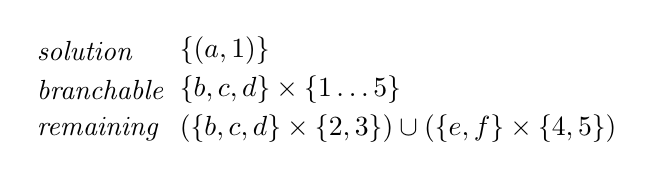
\begin{tikzpicture}[scale=0.33]
                    \node [anchor=west] (Ns) at (0, 3.5) { $\mathit{solution}$ };
                    \node [anchor=west] (Nb) at (0, 2) { $\mathit{branchable}$ };
                    \node [anchor=west] (Nr) at (0, 0.5) { $\mathit{remaining}$ };

                    \node [anchor=west] (Vs) at (5.5, 3.5) { $\{ (a, 1) \}$ };
                    \node [anchor=west] (Vb) at (5.5, 2) { $\{ b, c, d \} \times \{1 \ldots 5 \}$ };
                    \node [anchor=west] (Vr) at (5.5, 0.5) { $(\{ b, c, d \} \times \{ 2, 3 \}) \cup (\{ e, f\} \times \{ 4, 5 \})$ };
            \end{tikzpicture}
            \\[0.1cm]
            \stepcounter{stepcounter2}\roman{stepcounter2}) Initial problem &
            \stepcounter{stepcounter2}\roman{stepcounter2}) Search variables after guessing $a \mapsto 1$
            \\[0.4cm]
            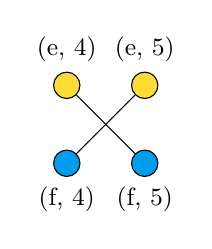
\begin{tikzpicture}[scale=0.33]
                    \node[draw, circle, fill=uofgsunshine, inner sep=0.5pt, font=\normalsize] (Me4) at (0, 3) {\phantom{0}};
                    \node[draw, circle, fill=uofgsunshine, inner sep=0.5pt, font=\normalsize] (Me5) at (3, 3) {\phantom{0}};
                    \node[draw, circle, fill=uofgcobalt, inner sep=0.5pt, font=\normalsize] (Mf4) at (0, 0) {\phantom{0}};
                    \node[draw, circle, fill=uofgcobalt, inner sep=0.5pt, font=\normalsize] (Mf5) at (3, 0) {\phantom{0}};

                    \node [above = 0 of Me4, font=\small] { \vphantom{0}(e, 4) };
                    \node [above = 0 of Me5, font=\small] { \vphantom{0}(e, 5) };
                    \node [below = 0 of Mf4, font=\small] { \vphantom{0}(f, 4) };
                    \node [below = 0 of Mf5, font=\small] { \vphantom{0}(f, 5) };

                    \draw (Me4) -- (Mf5);
                    \draw (Me5) -- (Mf4);
            \end{tikzpicture}
            &
            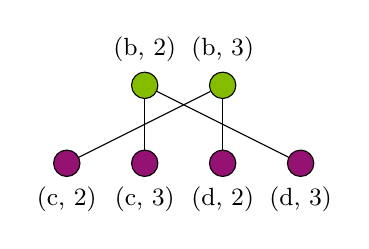
\begin{tikzpicture}[scale=0.33]
                    \node[draw, circle, fill=uofglawn, inner sep=0.5pt, font=\normalsize] (Mb2) at (3, 3) {\phantom{0}};
                    \node[draw, circle, fill=uofglawn, inner sep=0.5pt, font=\normalsize] (Mb3) at (6, 3) {\phantom{0}};
                    \node[draw, circle, fill=uofgthistle, inner sep=0.5pt, font=\normalsize] (Mc2) at (0, 0) {\phantom{0}};
                    \node[draw, circle, fill=uofgthistle, inner sep=0.5pt, font=\normalsize] (Mc3) at (3, 0) {\phantom{0}};
                    \node[draw, circle, fill=uofgthistle, inner sep=0.5pt, font=\normalsize] (Md2) at (6, 0) {\phantom{0}};
                    \node[draw, circle, fill=uofgthistle, inner sep=0.5pt, font=\normalsize] (Md3) at (9, 0) {\phantom{0}};

                    \node [above = 0 of Mb2, font=\small] { \vphantom{0}(b, 2) };
                    \node [above = 0 of Mb3, font=\small] { \vphantom{0}(b, 3) };
                    \node [below = 0 of Mc2, font=\small] { \vphantom{0}(c, 2) };
                    \node [below = 0 of Mc3, font=\small] { \vphantom{0}(c, 3) };
                    \node [below = 0 of Md2, font=\small] { \vphantom{0}(d, 2) };
                    \node [below = 0 of Md3, font=\small] { \vphantom{0}(d, 3) };

                    \draw (Mb2) -- (Mc3);
                    \draw (Mb2) -- (Md3);
                    \draw (Mb3) -- (Mc2);
                    \draw (Mb3) -- (Md2);
            \end{tikzpicture}
            \\[0.1cm]
            \stepcounter{stepcounter2}\roman{stepcounter2}) $\mathit{remaining} \setminus \mathit{branchable}$ &
            \stepcounter{stepcounter2}\roman{stepcounter2}) $\mathit{remaining} \cap \mathit{branchable}$
            \\
        };
    \end{tikzpicture}\\[0.3cm]\begin{tikzpicture}[scale=0.33]
        \matrix (m) [matrix of nodes] {
            \begin{tikzpicture}[scale=0.33]
                \node[draw, circle, fill=uofgsunshine, inner sep=0.5pt, font=\normalsize] (Me4) at (0, 0) {\phantom{0}};
                \node[draw, circle, fill=uofgsunshine, inner sep=0.5pt, font=\normalsize] (Me5) at (3, 0) {\phantom{0}};
                \node[draw, circle, fill=uofgcobalt, inner sep=0.5pt, font=\normalsize] (Mf4) at (6, 0) {\phantom{0}};
                \node[draw, circle, fill=uofgcobalt, inner sep=0.5pt, font=\normalsize] (Mf5) at (9, 0) {\phantom{0}};
                \node[draw, circle, fill=uofglawn, inner sep=0.5pt, font=\normalsize] (Mb2) at (12, 0) {\phantom{0}};
                \node[draw, circle, fill=uofglawn, inner sep=0.5pt, font=\normalsize] (Mb3) at (15, 0) {\phantom{0}};
                \node[draw, circle, fill=uofgthistle, inner sep=0.5pt, font=\normalsize] (Mc2) at (18, 0) {\phantom{0}};
                \node[draw, circle, fill=uofgthistle, inner sep=0.5pt, font=\normalsize] (Mc3) at (21, 0) {\phantom{0}};
                \node[draw, circle, fill=uofgthistle, inner sep=0.5pt, font=\normalsize] (Md2) at (24, 0) {\phantom{0}};
                \node[draw, circle, fill=uofgthistle, inner sep=0.5pt, font=\normalsize] (Md3) at (27, 0) {\phantom{0}};

                \node [above = 0 of Me4, font=\small, xshift=-0.5ex] { \vphantom{0}[[(e, 4), };
                \node [above = 0 of Me5, font=\small] { \vphantom{0}(e, 5)], };
                \node [above = 0 of Mf4, font=\small] { \vphantom{0}[(f, 4), };
                \node [above = 0 of Mf5, font=\small] { \vphantom{0}(f, 5)], };
                \node [above = 0 of Mb2, font=\small] { \vphantom{0}[(b, 2), };
                \node [above = 0 of Mb3, font=\small] { \vphantom{0}(b, 3)], };
                \node [above = 0 of Mc2, font=\small] { \vphantom{0}[(c, 2), };
                \node [above = 0 of Mc3, font=\small] { \vphantom{0}(c, 3), };
                \node [above = 0 of Md2, font=\small] { \vphantom{0}(d, 2), };
                \node [above = 0 of Md3, font=\small] { \vphantom{0}(d, 3)]]};
            \end{tikzpicture}
            \\[0.1cm]
            \stepcounter{stepcounter2}\roman{stepcounter2}) The resulting $\mathit{colourClasses}$ variable.
            \\
        };
    \end{tikzpicture}

    \caption{Solving a maximum common connected problem using an association graph. Suppose we
        have already mapped vertex $a$ to vertex $1$, giving the assignments on the right. Now we
        have two subgraphs to colour. We need two colours for $\mathit{remaining} \setminus
        \mathit{branchable}$, and we place these two colour classes first in the $\mathit{colourClasses}$
        variable. We can also colour $\mathit{remaining} \cap \mathit{branchable}$ using two
        colours, since we cannot simultaneously map $c$ to $2$ and $d$ to $3$, or vice-versa. Thus
        $\mathit{colourClasses}$ becomes a list of four colour classes, the first three containing
        two vertices each, and the last containing four vertices. This tells us that if we hope to
        extend the current common subgraph by another four vertices, we
        must pick one assignment from each of the four colour classes (which is not actually possible, so we
    see the bound here gives an overestimate). The algorithm thus guesses $d \mapsto 3$ as its next
assignment, and if that fails, $d \mapsto 2$, and so on; once $b \mapsto 3$ is reached, the bound
decreases by one, and if $f \mapsto 5$ were reached we would stop due to a lack of remaining
branchable vertices. }\label{figure:assocrestricted}
\end{figure}

It is not possible to determine connectedness from a raw association graph. However, we can take a
maximum clique algorithm and mimic the branching strategy if we have access to the underlying graphs
and can determine the ``meaning'' of the association graph vertices.

Most modern maximum clique algorithms for dense graphs use some variation of greedy graph colouring
as a bound---the underlying observation is that each vertex in a clique must be given a different
colour in a colouring, so if we can colour a subset of vertices using $k$ colours then a maximum
clique in this subset has at most $k$ vertices. However, the colouring is also used as a branching
heuristic: vertices are selected in reverse from their colour classes in turn, starting with the
last colour class created. Because of this coupling of branching and the bound (which is important
in practice because it mimics a ``smallest domain first'' branching heuristic if colour classes are
viewed as variables \cite{DBLP:conf/cp/McCreeshP14}), if we were to select only a subset of vertices for
branching at each stage inside a clique algorithm, we would lose completeness. Thus we must adapt
the bound to take into account restricted branching.

In \cref{algorithm:mccis} we present a clique-inspired algorithm which finds a maximum common
connected induced subgraph isomorphism via an
association graph. If the additional
branching restrictions are removed, the core of the algorithm is what Prosser
\cite{DBLP:journals/algorithms/Prosser12} calls the ``MCSa1'' variant of a series of algorithms due
to Tomita \textit{et al.}\
\cite{DBLP:conf/dmtcs/TomitaS03,DBLP:journals/jgo/TomitaK07,DBLP:conf/walcom/TomitaSHTW10}, using a
bitset encoding approach due to San Segundo \textit{et al.}\
\cite{DBLP:journals/cor/SegundoRJ11,DBLP:journals/ol/SegundoMRH13} (and we refer the reader to these
papers for implementation details on how to use bitsets and other data structures to implement the
colouring stage with very low constant factors).

We begin by building the association graph (\lineref{buildassoc}). The main part of the algorithm
then works by building up candidate cliques in the $\mathit{solution}$ variable, by recursive calls
to the $\mathit{search}$ procedure---starting from the empty set (\lineref{firstsearch}), each
recursive subcall adds one vertex to $\mathit{solution}$ (\lineref{addv}) in such a way that
$\mathit{solution}$ is always a clique which corresponds to a connected common subgraph. The
$\mathit{remaining}$ set contains the set of vertices which are adjacent to every vertex in
$\mathit{solution}$, and which have not yet been accepted or rejected (and so initially it contains
every vertex). The main loops in the $\FuncSty{search}$ procedure
(\twolinesref{outerloop}{innerloop}) have the effect of iterating over each vertex in this set in a
particular order---each vertex $v$ is selected in turn, and then a recursive call is made to
consider the effects of including $v$ in $\mathit{solution}$ (\lineref{recursesearch}), followed by
the next iteration where $v$ is instead rejected. When $v$ is accepted, we add it to the new
$\mathit{solution'}$ (\lineref{addvtosolution}), and create a new $\mathit{remaining'}$ containing
only the vertices in $\mathit{remaining}$ which are adjacent to $v$ (\lineref{filterremaining}).

The $\mathit{branchable}$ set contains the set of association graph vertices which correspond to
vertices adjacent to an already-accepted vertex in the first input graph---in constraint programming terms, it is the
set of assignments which could be made next which preserve connectedness. (Using only one of the two
input graphs is sufficient for correctness, and has the advantage that the $\FuncSty{connected}$
function may be implemented as a simple lookup into a precomputed array which maps each vertex in
the first input graph to a bitset.) At the top of search, this set is empty, and is not used (our
first vertex selection is special, and does not care about connectedness). At subsequent depths, we
may only accept vertices which are in this set, and if no such vertices remain then we return
immediately (\lineref{acceptbranchable}). When recursing, we extend $\mathit{branchable}$ with the
new vertices permitted by our acceptance of the branching $v$ (\lineref{addtobranchable}). Note that
we are assuming that inside the main loops, we encounter every vertex in $\mathit{remaining} \cap
\mathit{connected}$ before any vertex in $\mathit{remaining} \setminus \mathit{connected}$.

As we proceed, we keep track of the best solution we have found so far---this is stored in the
$\mathit{incumbent}$ variable (\twolinesref{incumbent}{newincumbent}). We use the incumbent,
together with a colour bound, to prune portions of the search space which cannot contain a better
solution. The colour bound operates as follows: at each entry to the $\FuncSty{search}$ procedure,
we produce a greedy colouring of the vertices in $\mathit{remaining}$ (\lineref{makecolours}). This
greedy colouring gives us a list of colour classes, each of which is a list of pairwise non-adjacent
vertices. The two loops (\twolinesref{outerloop}{innerloop}) then iterate over each colour class,
from last to first, and then over each vertex in that colour class, again from last to first.
(Rather than actually using a list of lists and removing items, this process should be implemented
using a pair of immutable flat arrays. This technique is described elsewhere
\cite{DBLP:conf/cp/McCreeshP14}, so we do not discuss it here.) Finally, if at any point the number
of remaining colour classes plus the number of vertices currently present in $\mathit{solution}$ is
not strictly greater than the size of the incumbent, then we may backtrack immediately
(\lineref{bound}).

Finally, we describe the colouring process. In conventional clique algorithms, a simple greedy
sequential colouring is used (possibly with the help of previous colourings to reduce the
computational cost \cite{DBLP:conf/lion/NikolaevBS15}, and possibly with shortcuts taken for certain
vertices \cite{DBLP:journals/cor/SegundoT14}, and possibly followed by a repair step to
improve the colouring \cite{DBLP:conf/walcom/TomitaSHTW10}, or stronger bounding rules based upon
MaxSAT inference \cite{DBLP:conf/ictai/LiFX13,DBLP:conf/lion/LiJX15,DBLP:journals/cor/SegundoNB15}).
Such colourings will not give us the required property that vertices in $\mathit{remaining} \cap
\mathit{connected}$ come last (so they are selected first by the reverse branching order). Thus we
produce two greedy sequential colourings, first considering the non-branching vertices in
$\mathit{remaining} \setminus \mathit{connected}$, followed by the branching vertices, and
concatenate them (\lineref{makecolours}). This produces a valid colouring, since we do not merge any
colour classes between the two stages, although it may use more colours than a single colouring
would.

Our $\FuncSty{colour}$ procedure is the same as the bit-parallel algorithm introduced by San Segundo
\textit{et al.}\ \cite{DBLP:journals/cor/SegundoRJ11}. While we have remaining vertices to colour
(\lineref{whileuncoloured}), we start a new colour class (\lineref{newcolourclass}), and then
repeatedly pick a legal vertex to add to that colour class (\lineref{addtocolourclass}).  The
selection of the next vertex to colour (\lineref{selectvtocolour}) may be performed efficiently in
hardware if the association graph is permuted to be in degree order at the top of search. (Other
initial vertex orderings have been considered on general clique problems
\cite{DBLP:journals/algorithms/Prosser12,DBLP:conf/lion/SegundoLB14}; it is possible that special
properties of the association graph could be exploited in this step.)

\subsection{Experimental Evaluation}

\paragraph{Connected, Undirected, 33\% Labelled} \cref{figure:connected-undir33} Above two seconds,
    the clique approach dominates except for three instances, and there is only one instance which
    the constraint programming model can solve but the clique model cannot (?? is this an EHP and does parallel get rid
    of it?). The clique model is unable to solve only ??  instances within one hour, ?? all of which
    have 90 or 100 vertices.  On the other hand, for trivial instances, the clique approach is often
    expensive due to the association graph construction.

\paragraph{Connected, Undirected, Unlabelled} \cref{figure:connected-plain}, looks like the clique
approach doesn't do so well\ldots

?? My gut feeling is that if we have edge labels, the clique model wins, and if we don't, it's
likely to lose. So maybe I should run some experiments with vertex labels but not edge labels to
test this.

\paragraph{By family} ?? Break this down more by family, size, etc.

\paragraph{Does connected make instances easier or harder?} We could plot connected vs not connected
difficulties, and result sizes?


\begin{figure}[p]
    \centering
    \input{gen-graph-connected-undir33}
    \caption{Clique versus constraint programming, connected, undirected, 33\% labelled, up to 100 vertices. On the top,
        the cumulative number of instances solved by each approach, in under a certain time. On the
        bottom, the association graph approach compared to the constraint programming approach with
        both branching and filtering.} \label{figure:connected-undir33}
\end{figure}

\begin{figure}[p]
    \centering
    \input{gen-graph-connected-undir33-breakdown}
    \caption{Clique versus constraint programming, connected, undirected, 33\% labelled, broken down by family.}
        \label{figure:connected-undir33-breakdown}
\end{figure}

\begin{figure}[p]
    \centering
    \input{gen-graph-connected-plain}
    \caption{Clique versus constraint programming, connected, undirected, unlabelled, up to 35 vertices. On the top, the
        cumulative number of instances solved by each approach, in under a certain time. On the
        bottom, the association graph approach compared to the constraint programming approach
    with both branching and filtering.}
\label{figure:connected-plain}
\end{figure}

\begin{figure}[p]
    \centering
    \input{gen-graph-connected-plain-breakdown}
    \caption{Clique versus constraint programming, connected, undirected, unlabelled, broken down by family.}
        \label{figure:connected-plain-breakdown}
\end{figure}

\subsection{Parallel Search}

\cite{DBLP:conf/ictai/MinotNS15}

\section{Conclusion}

Some immoral perspectives on closely coupling branching with a particular constraint. Whether this
is useful for other things, like ASP.

We haven't discussed partial subgraphs, or connected directed.

Possibly portfolios.

Better instances.

\bibliographystyle{splncs}
\bibliography{paper}

\end{document}

